%%%%%%%%%%%%%%%%%%%%%%%%%%%%%%%%%%%%%%%%%%%%%%%%%%%%%%%%%%%
% | - Active Learning Machine Learning Results
% %%%%%%%%%%%%%%%%%%%%%%%%%%%%%%%%%%%%%%%%%%%%%%%%%%%%%%%%%
%
% Notes:
%   - QUESTION Is there any physical intuition that we can gleam from the fingerprints?
%     * Probably not important
%   - QUESTION What did @Chris mean by this? "Computed amorphous phase to define synthesizability"
%     * ANSWER: Referring to Murat's paper R85
%     * I don't think we can take advantage of this since there is no amorphous data for IrO3
% Mention that we have ~15 metastable structures inbetween rutile and anatase IrO2
% __|
%%%%%%%%%%%%%%%%%%%%%%%%%%%%%%%%%%%%%%%%%%%%%%%%%%%%%%%%%%%



% %%%%%%%%%%%%%%%%%%%%%%%%%%%%%%%%%%%%%%%%%%%%%%%%%%%%%%%%%
% | - PARAGRAPH HEADER
% Intro/transition paragraph
% __|
% %%%%%%%%%%%%%%%%%%%%%%%%%%%%%%%%%%%%%%%%%%%%%%%%%%%%%%%%%
% | - PARAGRAPH BODY
%
We now demonstrate the AL algorithm by applying it to the discovery of stable and unique polymorphs of \IrOtwo and \IrOthree.
% We next utilized the active learning scheme to discover of the most stable forms of \IrOtwo and \IrOthree.
%
Since the algorithm is applied to each stoichiometry individually, we will only illustrate the results for \IrOthree, a comparatively less explored oxide
% and because both cases demonstrate the efficacy of the algorithm equally well, we will focus on walking through the algorithm for the more novel \IrOthree stoichiometry.
%
We will briefly touch on the results for \IrOtwo at the end and refer the reader to the Supporting Information for further information.
% __|
%%%%%%%%%%%%%%%%%%%%%%%%%%%%%%%%%%%%%%%%%%%%%%%%%%%%%%%%%%%


% %%%%%%%%%%%%%%%%%%%%%%%%%%%%%%%%%%%%%%%%%%%%%%%%%%%%%%%%%
% | - PARAGRAPH HEADER
% Results for IrO3
% AL results for IrO3
%   * Introduce the convergence plots
%   * The GP becomes more accurate as more DFT is acquired
%   * The GP can start to recognize the low energy systems after minimal DFT
%   *
% We need to call them something else than "convergence plots" (bad name)
% __|
% %%%%%%%%%%%%%%%%%%%%%%%%%%%%%%%%%%%%%%%%%%%%%%%%%%%%%%%%%
% | - PARAGRAPH BODY
%
The application of the AL algorithm to identifying the stable polymorphs of the \IrOthree candidate space is shown in
Figure~\ref{fig:iro3_al}a,
which shows a sequence of snapshots of the AL routine at different generations.
%
% COMBAK Why are we sorting? Explain
Each plot reports the predicted (hollow grey) and DFT-derived (solid red) formation enthalpies (\DHf) ($y$-axis) for each structure sorted by stability ($x$-axis).
%
As the algorithm acquires DFT \DHf values, the GP model becomes more accurate, as evidenced by the decreasing uncertainties when comparing the initial generations to the latter generations of the AL (\ref{fig:iro3_al}a.i-v).
%
At the top of each subplot of Figure~\ref{fig:iro3_al}a the identity of ten most stable polymorphs is tracked.
%
Initially, the ten most stable structures are randomly distributed across the entire candidate space due to the insufficiently trained GP model.
%
After only three generations (Figure~\ref{fig:iro3_al}a.ii) the GP model is sufficiently accurate to identify all top ten of the most stable polymorphs as being low in energy.
%
By the fifth generation (\num{30} DFT relaxation) \num{4/10} of the most stable polymorphs have been acquired,
including the globally stable phase of \IrOthree.
%
% COMBAK Does this syntax work with num?
After an additional nine generations of the AL
(Figure~\ref{fig:iro3_al}a.iv),
the algorithm has acquired all but one of the top ten low energy structures.
% __|
%%%%%%%%%%%%%%%%%%%%%%%%%%%%%%%%%%%%%%%%%%%%%%%%%%%%%%%%%%%


% %%%%%%%%%%%%%%%%%%%%%%%%%%%%%%%%%%%%%%%%%%%%%%%%%%%%%%%%%
% | - PARAGRAPH HEADER
% PARAGRAPH ABOUT STRUCTURES FOUND
% How to balance this with the next section that has more details on structural stuff?
% __|
% %%%%%%%%%%%%%%%%%%%%%%%%%%%%%%%%%%%%%%%%%%%%%%%%%%%%%%%%%
% | - PARAGRAPH BODY
%
TEMP PARAGRAPH ON STRUCTURES FOUND
% __|
%%%%%%%%%%%%%%%%%%%%%%%%%%%%%%%%%%%%%%%%%%%%%%%%%%%%%%%%%%%


% %%%%%%%%%%%%%%%%%%%%%%%%%%%%%%%%%%%%%%%%%%%%%%%%%%%%%%%%%
% | - PARAGRAPH HEADER
% Performance of model
% __|
% %%%%%%%%%%%%%%%%%%%%%%%%%%%%%%%%%%%%%%%%%%%%%%%%%%%%%%%%%
% | - PARAGRAPH BODY
%
Figure~\ref{fig:iro3_al}c reports the quantity of the most stable ten systems acquired as a function of DFT calculations for the AL algorithm with the GP-UCB acquisition function and a baseline random acquisition scheme.
%
The results of Figure~\ref{fig:iro3_al}c are averaged over 100 independent runs of AL algorithms with the 1 sigma standard deviation between these runs shown.
%
% COMBAK Pick better point to compare
Overall, the GP-UCB runs outperform the random acquisition runs, with only \num{50} DFT calculations on average needed to discover \num{7} of the \num{10} most stable systems.
%
This is compared to the \num{157} DFT calculations needed to discover \num{7/10} most stable polymorphs for the AL utilizing a random acquisition.
% __|
%%%%%%%%%%%%%%%%%%%%%%%%%%%%%%%%%%%%%%%%%%%%%%%%%%%%%%%%%%%


% =========================================================
% FIGURE ==================================================
% =========================================================
% | - Figure | IrO3 Convergence Plot
\begin{figure*}[!htb]
    \centering
    \makebox[\textwidth][c]{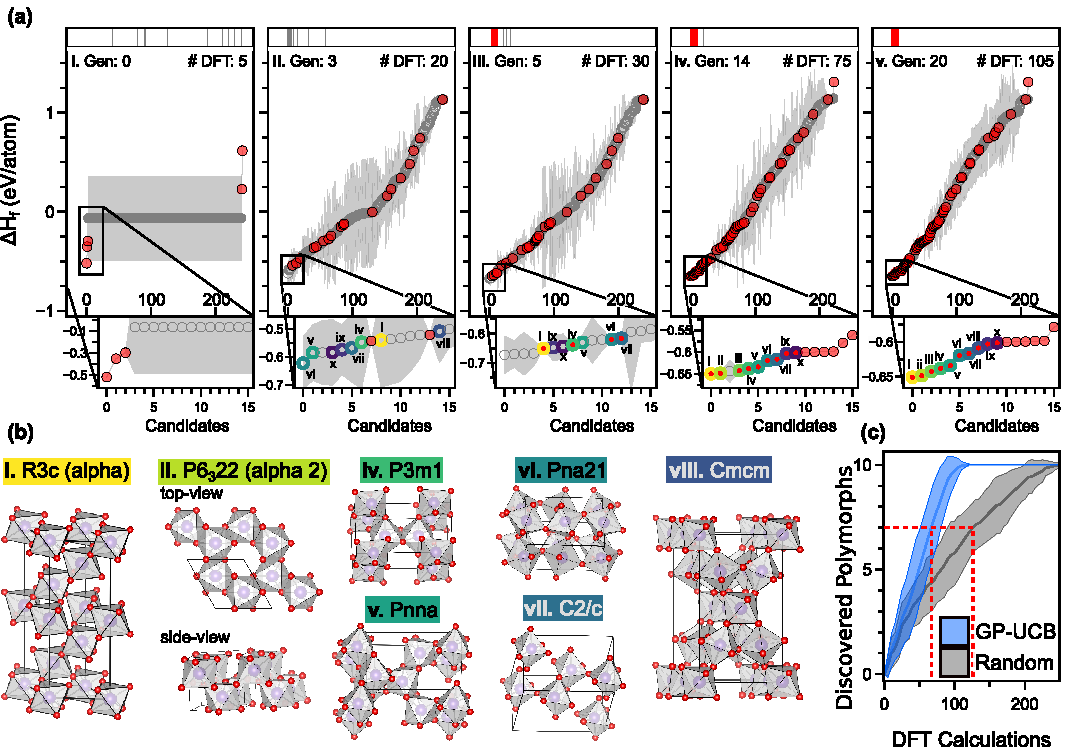
\includegraphics[width=\textwidth,height=\textheight,keepaspectratio]
        {02_figures/ml_convergence_plots/test_iro3_al.pdf}
    }
    \caption{\label{fig:iro3_al}
        % (a) %%%%%%%%%%%%%%%%%%%%%%%%%%%%%%%%%%%%%%%%%%%%%%%%%%%%%
        %
        (a) The state of the AL algorithm at five generations.
        %
        The enthalpy of formation per atom (\DHf) is plotted, ordered from most to least stable, against all \IrOthree candidates.
        %
        The number of DFT training points the GP model at each generation is displayed.
        %
        Hollow grey markers indicate a GP model predicted \DHf while red points indicate a DFT-computed quantity.
        %
        GP uncertainty estimates corresponding to one sigma are shown for all predictions.
        %
        At the top of subplots a.i through a.v, the x-axis positions of the ten most stable polymorphs are tracked at each generation by either red (acquired) or grey (not acquired) vertical lines.
        %
        Insets of the low energy region for each generation is displayed below each subplot.
        %
        The top ten most stable systems are colored and labeled to indicate their identity.
        % (b) %%%%%%%%%%%%%%%%%%%%%%%%%%%%%%%%%%%%%%%%%%%%%%%%%%%%%
        %
        (b) Crystal structures of the \num{8} most stable \IrOthree polymorphs.
        %
        The third most stable polymorphs is excluded since it is a combination of the first and second most stable systems.
        % (c) %%%%%%%%%%%%%%%%%%%%%%%%%%%%%%%%%%%%%%%%%%%%%%%%%%%%%
        %
        (c) The number of most stable \num{10} polymorphs of \IrOthree that are discovered as a function of the number of DFT bulk relaxations,
        averaged over \num{100} independent runs of the AL algorithm using the GP-UCB acquisition criteria (blue) and a random acquisition (grey).
        %
        The error bars indicate the standard deviation over \num{100} runs.
        %
        Red guide lines are displayed to show how many DFT calculations are needed to discover \num{7/10} of most stable polymorphs for the GP-UCB and random acquisition.
    }
\end{figure*}

% (b) %%%%%%%%%%%%%%%%%%%%%%%%%%%%%%%%%%%%%%%%%%%%%%%%%%%%%
% (b) Parity plot of the final ML models for \IrOtwo and \IrOthree predicting on either the pre-optimized (grey) or the post-optimized structures of \IrOtwo and \IrOthree.
% (c) %%%%%%%%%%%%%%%%%%%%%%%%%%%%%%%%%%%%%%%%%%%%%%%%%%%%%
% (c) Zoomed inset of the 6th generation of the AL loop.

% __| =====================================================
% =========================================================


% %%%%%%%%%%%%%%%%%%%%%%%%%%%%%%%%%%%%%%%%%%%%%%%%%%%%%%%%%
% | - PARAGRAPH HEADER
% Discussion on performance of the AL routine
% __|
% %%%%%%%%%%%%%%%%%%%%%%%%%%%%%%%%%%%%%%%%%%%%%%%%%%%%%%%%%
% | - PARAGRAPH BODY
We next evaluate the performance of the \IrOtwo and \IrOthree GP regression models trained on the full DFT dataset (corresponding to the final AL generation).
%
Figure~\ref{fig:parity} plots the GP model predicted \DHf against the DFT-computed values for two special cases.
%
Case 1) shows the predictions on the pre-optimized structural features, as is done in the regular operation of the algorithm when acquiring new structures and
case 2) shows the prediction of the same model onto the post-DFT optimized features (blue).
%
It is evident from the parity plot that the GP model is not accurate in quantitatively predicting the DFT formation energy of the candidate space using the pre-optimized fingerprints,
with a MAE of \mytilde\num{1.5} eV/atom.
%
The largest errors are highly skewed towards the more unstable systems.
%
The same GP model does comparatively much better at predicting the formation energies of post-DFT optimized structures with an MAE of \mytilde\num{0.2} eV/atom,
roughly 100 meV/atom larger than model reported by Ward \latin{et al.}, which was trained on hundreds of thousands of DFT bulk calculations and reached an MAE of 0.8 eV/atom.
%
% __|
%%%%%%%%%%%%%%%%%%%%%%%%%%%%%%%%%%%%%%%%%%%%%%%%%%%%%%%%%%%


% %%%%%%%%%%%%%%%%%%%%%%%%%%%%%%%%%%%%%%%%%%%%%%%%%%%%%%%%%
% | - PARAGRAPH HEADER
% DISCUSS PERFORMANCE AND STRUCTURAL SHIFT
% __|
% %%%%%%%%%%%%%%%%%%%%%%%%%%%%%%%%%%%%%%%%%%%%%%%%%%%%%%%%%
% | - PARAGRAPH BODY
The fact that our models,
trained on orders of magnitude less data than those of Ward \latin{et al.},
achieve errors on par with those of Ward \latin{et al.},
is due to the fact that we are training and predicting on a space whose properties are very narrowly constrained, while Ward \latin{et al.} is predicting on structures whose elements span the entire periodic table.
%
This drastic decrease in prediction error is not surprising since the post-DFT fingerprints directly corresponds to the target DFT energies.
%
Our comparison in \ref{fig:parity} is to show that our model's inaccuracies are due to the large degree of structural drift that occurs after DFT relaxation, and the extent of this drift is not known \latin{a priori}.
%
Structures that are initialized in high energy configurations will therefore have high predicted \DHf,
and will then reconfigure into a lower nearby configuration, resulting in lower final energy and a large discrepancy between the predicted and final energies.
%
% \textbf{do determine the reason for this we did TEMP...}
Interestingly, despite the inaccuracy of predictions on unrelaxed structures the algorithm appears to perform well at discovering \num{7/10} of the most stable candidates after only \num{35} DFT calculations.
%
% \textbf{How do you know this?  This is in the section?  If it is you need to say it will be discussed in the next section here.}
The reason for this is that the pre-optimized structures that are similar enough to the most stable final equilibrium structures will not restructure considerably, meaning that their predicted formation energies will be close enough (and low enough) to be quickly picked up by the acquisition criteria.
% __|
%%%%%%%%%%%%%%%%%%%%%%%%%%%%%%%%%%%%%%%%%%%%%%%%%%%%%%%%%%%


% =========================================================
% FIGURE ==================================================
% | - Figure | IrO2/3 Parity Plot
\begin{figure*}[!htb]
\centering
\makebox[\textwidth][c]{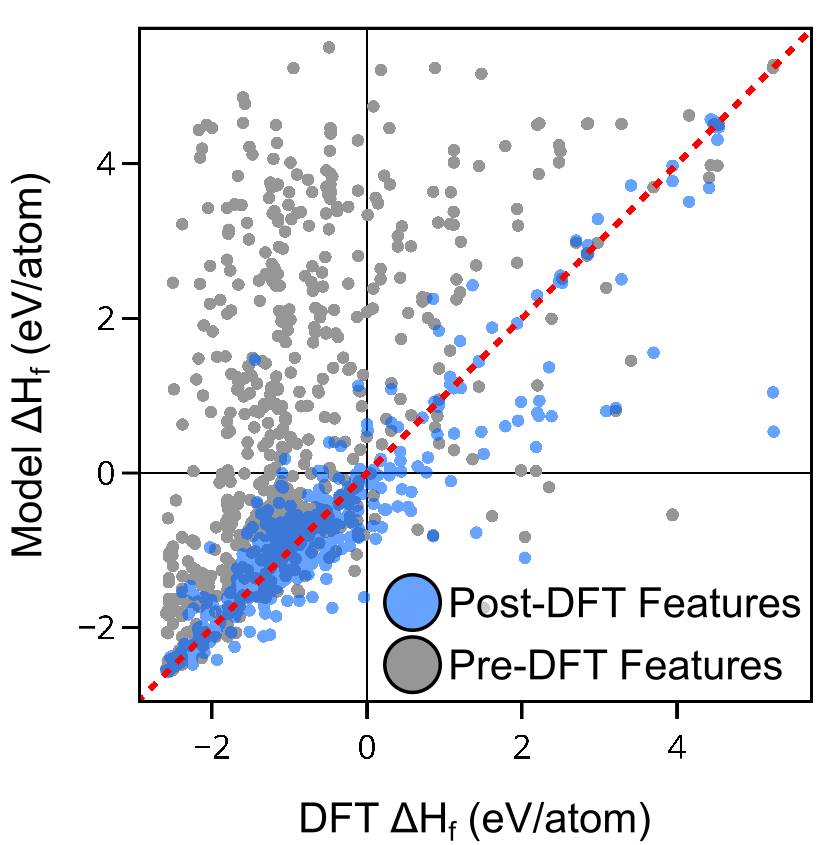
\includegraphics[]
{02_figures/parity_plot.png}
}
\caption{\label{fig:parity}
%
Parity plot of the final ML models for \IrOtwo and \IrOthree predicting on either the pre-optimized (grey) or the post-optimized structures of \IrOtwo and \IrOthree.
}
\end{figure*}
% __|
% =========================================================
